%style input
\documentclass[runningheads]{llncs}

\newif\ifLNCSVER
%\LNCSVERtrue
\LNCSVERfalse

\ifLNCSVER

\else
  \usepackage[letterpaper,hmargin=1.25in,vmargin=1.0in]{geometry}
\fi



%\usepackage[letterpaper,hmargin=1.25in,vmargin=1.25in]{geometry}
\setcounter{tocdepth}{3}
\usepackage{graphicx}
\usepackage{amsmath,url,bm,amssymb,latexsym,multirow,multicol,xspace,subfigure,afterpage,lscape,booktabs,cancel,dashbox}
\usepackage{algorithm,algpseudocode}
\usepackage{colortbl}
\usepackage{comment,multirow}
\usepackage[normalem]{ulem}
\usepackage{hyperref}
\usepackage{todonotes}
\usepackage{tikz,pgfplots}
\usepackage{subfigure}
\usepackage{autobreak}
\usepackage{mathtools}


\renewcommand{\floatpagefraction}{0.95}
\renewcommand{\topfraction}{0.95}

\usepackage{lineno}

\usepackage{listings}
\lstset{
	backgroundcolor=\color{white},   % choose the background color; you must add \usepackage{color} or \usepackage{xcolor}; should come as last argument
	basicstyle=\ttfamily\scriptsize,        % the size of the fonts that are used for the code
	breakatwhitespace=false,         % sets if automatic breaks should only happen at whitespace
	breaklines=true,                 % sets automatic line breaking
	captionpos=b,                    % sets the caption-position to bottom
	commentstyle=\color{green},    % comment style
	deletekeywords={...},            % if you want to delete keywords from the given language
	escapeinside={\%*}{*)},          % if you want to add LaTeX within your code
	extendedchars=true,              % lets you use non-ASCII characters; for 8-bits encodings only, does not work with UTF-8
	firstnumber=1,                % start line enumeration with line 1000
	frame=single,	                   % adds a frame around the code
	keepspaces=true,                 % keeps spaces in text, useful for keeping indentation of code (possibly needs columns=flexible)
	keywordstyle=\color{blue},       % keyword style
	language=Python,                 % the language of the code
	morekeywords={*,...},            % if you want to add more keywords to the set
	numbers=left,                    % where to put the line-numbers; possible values are (none, left, right)
	numbersep=5pt,                   % how far the line-numbers are from the code
	numberstyle=\tiny\color{gray}, % the style that is used for the line-numbers
	rulecolor=\color{black},         % if not set, the frame-color may be changed on line-breaks within not-black text (e.g. comments (green here))
	showspaces=false,                % show spaces everywhere adding particular underscores; it overrides 'showstringspaces'
	showstringspaces=false,          % underline spaces within strings only
	showtabs=false,                  % show tabs within strings adding particular underscores
	stepnumber=1,                    % the step between two line-numbers. If it's 1, each line will be numbered
	%stringstyle=\color{mauve},     % string literal style
	tabsize=2,	                   % sets default tabsize to 2 spaces
	title=\lstname                   % show the filename of files included with \lstinputlisting; also try caption instead of title
}

\renewcommand{\floatpagefraction}{0.95}
\renewcommand{\topfraction}{0.95}

\makeatletter
\def\add(#1,#2){{%
		\newcount\@a \@a = #1 \relax
		\advance \@a by #2 \relax
		\the\@a
}}
\makeatother

%\newcommand*\patchAmsMathEnvironmentForLineno[1]{%
%	\expandafter\let\csname old#1\expandafter\endcsname\csname #1\endcsname
%	\expandafter\let\csname oldend#1\expandafter\endcsname\csname end#1\endcsname
%	\renewenvironment{#1}%
%	{\linenomath\csname old#1\endcsname}%
%	{\csname oldend#1\endcsname\endlinenomath}}%
%\newcommand*\patchBothAmsMathEnvironmentsForLineno[1]{%
%	\patchAmsMathEnvironmentForLineno{#1}%
%	\patchAmsMathEnvironmentForLineno{#1*}}%
%\AtBeginDocument{%
%	\patchBothAmsMathEnvironmentsForLineno{equation}%
%	\patchBothAmsMathEnvironmentsForLineno{align}%
%	\patchBothAmsMathEnvironmentsForLineno{flalign}%
%	\patchBothAmsMathEnvironmentsForLineno{alignat}%
%	\patchBothAmsMathEnvironmentsForLineno{gather}%
%	\patchBothAmsMathEnvironmentsForLineno{multline}%
%}
%\linenumbers

\usepackage{color}
\newcommand{\yt}[1]{\textcolor{red}{[{\bf Yosuke:} #1]}}
\newcommand{\yh}[1]{\textcolor{red}{[{Yonglin:} #1]}}
\newcommand{\qw}[1]{\textcolor{red}{[{Qingju:} #1]}}
%\newcommand{\discuss}[1]{\textcolor{red}{#1}}
\newcommand{\rc}[1]{\textcolor{red}{#1}}

\algdef{SE}[DOWHILE]{Do}{doWhile}{\algorithmicdo}[1]{\algorithmicwhile\ #1}

%\newtheorem{example}{Example}
\newtheorem{assumption}{Assumption}
\newtheorem{hypothesis}{Hypothesis}
\newtheorem{statement}{Statement}
%\newtheorem{question}{Open Question}

%
\newcommand{\gitaddress}{\url{https://github.com/ysktodo/milp-three-subset-wo-unknown}\xspace}

%
\newcommand{\seti}{\mathbb{X}}
\newcommand{\seto}{\mathbb{Y}}

%newcommand
%\newcommand{\A}{{\cal A}}
%\newcommand{\B}{{\cal B}}
%\newcommand{\C}{{\cal C}}
\newcommand{\D}{{\cal D}}
\newcommand{\T}{{\cal T}}

\DeclareMathOperator{\Prob}{Pr}

\newcommand{\F}{\mathbb{F}}
%\newcommand{\U}{{\cal U}}
\newcommand{\Sbox}{S-box\xspace}
\newcommand{\Sboxes}{S-boxes\xspace}
\newcommand{\etal}{{et al.}\xspace}
\newcommand{\eg}{{e.g.}\xspace}
\newcommand{\ie}{{i.e.}\xspace}
\newcommand{\st}{{s.t.}\xspace}

\newcommand{\ACORN}{\textsc{ACORN}\xspace}
\newcommand{\LUFFA}{{\it Luffa}\xspace}
\newcommand{\PHOTON}{\texttt{PHOTON}\xspace}
\newcommand{\LED}{\texttt{LED}\xspace}
\newcommand{\KECCAK}{\textsc{Keccak}\xspace}
\newcommand{\SQUARE}{\textsc{Square}\xspace}
\newcommand{\ANUBIS}{\textsc{Anubis}\xspace}
\newcommand{\WHIRLPOOL}{\textsc{Whirlpool}\xspace}
\newcommand{\GROESTL}{Gr{\o}stl\xspace}
\newcommand{\NOEKEON}{\textsc{Noekeon}\xspace}
\newcommand{\SKINNY}{\texttt{SKINNY}\xspace}
\newcommand{\MYSTERION}{\textsf{Mysterion}\xspace}
\newcommand{\lilliput}{\textsc{Lilliput}\xspace}
\newcommand{\SPARX}{\textsc{Sparx}\xspace}

\newcommand{\SIMON}{\textsc{Simon}}
\newcommand{\SIMECK}{\textsf{Simeck}}

\newcommand{\TRIVIUM}{\textsc{Trivium}\xspace}


\newcommand*{\NL}[1]{( b_{t+\add(#1,3)}b_{t+\add(#1,67)} + b_{t+\add(#1,11)}b_{t+\add(#1,13)} + b_{t+\add(#1,17)}b_{t+\add(#1,18)} + b_{t+\add(#1,27)}b_{t+\add(#1,59)} + b_{t+\add(#1,40)}b_{t+\add(#1,48)} + b_{t+\add(#1,61)}b_{t+\add(#1,65)} + b_{t+\add(#1,68)}b_{t+\add(#1,84)} \\ & \quad+ b_{t+\add(#1,88)}b_{t+\add(#1,92)}b_{t+\add(#1,93)}b_{t+\add(#1,95)} + b_{t+\add(#1,22)}b_{t+\add(#1,24)}b_{t+\add(#1,25)} + b_{t+\add(#1,70)}b_{t+\add(#1,78)}b_{t+\add(#1,82)} )}

\newcommand{\grain}{Grain-128\xspace}
\newcommand{\graina}{Grain-128a\xspace}
\newcommand{\grainv}{Grain-v1\xspace}
\newcommand*{\ls}[1]{L^{(#1)}}
\newcommand*{\lsp}[1]{s'^{(#1)}}
\newcommand*{\ns}[1]{N^{(#1)}}
\newcommand{\tz}{\mathbb{T}_z}
\newcommand{\tb}{\mathbb{T}_b}
\newcommand*{\mask}[1]{\Lambda_{#1}}
\newcommand{\set}{\mathbb{S}}

\newcommand{\GF}{\mathrm{GF}}
\newcommand{\mat}{F}
\newcommand*{\A}[1]{A_{#1}}
\newcommand*{\trans}[1]{{}^\mathrm{T}\!{#1}}

\newcommand*{\dl}[1]{\cancel{#1}}

%\usepackage{setspace}
%\setstretch{2}
\renewcommand{\algorithmicrequire}{\textbf{Input:}}
\renewcommand{\algorithmicensure}{\textbf{Output:}}

        \begin{document}
% start of an individual contribution
\mainmatter
% first the title is needed
\title{State-Recovery Attacks on A5/1 with Negligible Memory Complexities}
\author{Yonglin Hao\inst{1}\thanks{\email{haoyonglin@yeah.net} }
\and
Bin Zhang \inst{1,2,3,4}}
\institute{
	State Key Laboratory of Cryptology, P.O. Box 5159, Beijing 100878, China
\and
	TCA, SKLCS, Institute of Software, Chinese Academy of Sciences
\and
University of Chinese Academy of Sciences, Beijing, 100049, China
\and
State Key Laboratory of Information Security, Institute of Information Engineering,
Chinese Academy of Sciences
%\and
%	FHNW, Windisch, Switzerland, \email{willimeier48@gmail.com} \and
%	NTT Secure Platform Laboratories, Tokyo 180-8585, Japan, \email{yosuke.todo.xt@hco.ntt.co.jp} \and
%	SnT, University of Luxembourg, Esch-sur-Alzette, Luxembourg, \email{qingju.wang@uni.lu}
}
\maketitle


%\input{introduction_abst}

%\pagewiselinenumbers



%%%%%%%%%%%%%%%%%%%%%%%%%%%%%%%%%%%%%%%%%%%%%%%%%%%%%%%%%%%%%%%%%%%%%%%%%%%%%%%%%%%%%%%%%
%%%%%%%%%%%%%%%%%%%%%%%%%%%%%%%%%%%%%   Abstract   %%%%%%%%%%%%%%%%%%%%%%%%%%%%%%%%%%%%%%
%%%%%%%%%%%%%%%%%%%%%%%%%%%%%%%%%%%%%%%%%%%%%%%%%%%%%%%%%%%%%%%%%%%%%%%%%%%%%%%%%%%%%%%%%
\begin{abstract}
At Asiacrypt 2019, Zhang \etal proposed a state recovery attack on A5/1.
They divide the 64-bit A5/1 state into a CP part and a RP part, and recover them separately with overall time \& memory complexities around $2^{30}$.
But such an attack has never been fully implemented leaving its correctness unknown.

In this paper, we propose a series of state-recovery attacks on A5/1 with negligible memory complexities.
The main idea is based on a move-guessing technique and we maintain a system of linear bit conditions for distinguishing the correct state from the wrong ones.
The memory complexity is just thousands of bits which is negligible.
The time complexity can be as low as $2^{43.91}$ and the data complexity is only 32 bits.
The success probability is 100\%.

In addition to proposing our own attack, we revisit Zhang \etal's attack as well.
We fully implement the CP-recovery process of their attack and experimentally evaluate complexities of RP-recovery process as well.
We verify the incorrectness of Zhang \etal's attack: their complexities are far too optimistic and several crucial parameters are wrongly evaluated due to their incorrect implementations.
As a remedy, we provide detailed analysis along with correct complexity evaluations.
\keywords{stream ciphers, A5/1, guess-and-determine}
\end{abstract}

\section{Introduction}
We analyze the attack given by Bin Zhang in \cite{AC:Zhang19} only to find that the complexities given in \cite{AC:Zhang19} are far too optimistic.
As a remedy, we give detailed analysis to all the possible tradeoffs in the guess-and-determine attacks on A5/1 and give the best practical attack requiring simple $2^{44.60}$ computations and a negligible memory complexity.


\section{Preliminary}
In the 1st part of this section, we give a brief introduction to the keystream generation phase of the A5/1 stream cipher.
Then, in the 2nd part, we review the general process of Zhang \etal's attack in \cite{AC:Zhang19}.
\subsection{The Keystream Generation Procedure of A5/1}\label{sec:KSMA51}
A5/1 has a 64-bit internal state consisting of 3 registers of sizes 19, 22, 23 respectively.
We denote the 64-bit state at time $t$ ($t=0,1,2,\ldots$) as
\begin{equation}\label{eq:StateAndRi}
\begin{aligned}
   \vec s^t= & (\vec{R1}^t, \vec{R2}^t, \vec{R3}^t)\\
     =& (\vec{s}^t[0,\ldots, 18],\vec{s}^t[19,\ldots, 40],\vec{s}^t[41,\ldots, 63])\\
     =&(\vec{R1}^t[0,\ldots,18],\vec{R2}^t[0,\ldots, 21],\vec{R3}^t[0,\ldots,22])
\end{aligned}
\end{equation}
Before generating the output bit $z_t$, A5/1 round function will update the internal state $\vec{s}^t\rightarrow \vec{s}^{t+1}$ in a stop-and-go manner as follows:
\begin{enumerate}
  \item Compute $maj_t$ as
\begin{equation}\label{eq:Majt}
\begin{aligned}
  maj_t=&(\vec{R1}^t[8]\cdot \vec{R2}^t[10])\oplus (\vec{R1}^t[8]\cdot \vec{R3}^t[10])\oplus (\vec{R2}^t[10]\cdot \vec{R3}^t[10])\\
  =&(\vec{s}^t[8]\cdot \vec{s}^t[29])\oplus (\vec{s}^t[8]\cdot \vec{s}^t[51])\oplus (\vec{s}^t[29]\cdot \vec{s}^t[51])
\end{aligned}
\end{equation}
  \item If $\vec{R1}^t[8]=\vec{s}^t[8]\neq maj_t$, $\vec{R1}^{t+1}\leftarrow \vec{R1}^{t}$, otherwise, call $\tt{updateR1}$ as follows:
  \begin{equation}\label{eq:UpdateR1}
    \vec{R1}^{t+1}[i]\leftarrow\left\{
    \begin{aligned}
      &\vec{R1}^t[i-1]\quad i\in [1,18]\\
      &\vec{R1}^t[18]\oplus \vec{R1}^t[17]\oplus \vec{R1}^t[16]\oplus \vec{R1}^t[13]
    \end{aligned}
    \right.
  \end{equation}
  \item If $\vec{R2}^t[10]=\vec{s}^t[29]\neq maj_t$, $\vec{R2}^{t+1}\leftarrow \vec{R2}^t$, otherwise, call $\tt{updateR2}$ as follows:
    \begin{equation}\label{eq:UpdateR2}
    \vec{R2}^{t+1}[i]\leftarrow\left\{
    \begin{aligned}
      &\vec{R2}^t[i-1]\quad i\in [1,21]\\
      &\vec{R2}^t[21]\oplus \vec{R2}^t[20]
    \end{aligned}
    \right.
  \end{equation}
    \item If $\vec{R3}^t[10]=\vec{s}^t[51]\neq maj_t$, $\vec{R3}^{t+1}\leftarrow \vec{R3}^t$, otherwise, call $\tt{updateR3}$ as follows:
    \begin{equation}\label{eq:UpdateR3}
    \vec{R3}^{t+1}[i]\leftarrow\left\{
    \begin{aligned}
      &\vec{R3}^t[i-1]\quad i\in [1,22]\\
      &\vec{R3}^t[22]\oplus \vec{R3}^t[21]\oplus \vec{R3}^t[20]\oplus \vec{R3}^t[7]
    \end{aligned}
    \right.
  \end{equation}
\end{enumerate}
Then, the output keystream bit $z_t$ is generated as
\begin{equation}\label{eq:OutputZ}
\begin{aligned}
  z_t=&\vec{R1}^{t+1}[18]\oplus \vec{R2}^{t+1}[21]\oplus \vec{R3}^{t+1}[22]\\
  =&\vec{s}^{t+1}[18]\oplus \vec{s}^{t+1}[40]\oplus \vec{s}^{t+1}[63]
\end{aligned}
\end{equation}
In the remainder of this paper, we uniformly use $\vec{s}^t[i]$ to represent the $i$-th bit of the whole state and avoid using $\vec{R1}[j],\vec{R2}[k],\vec{R3}[\ell]$'s.

\subsection{Zhang \etal's Attack in \cite{AC:Zhang19}}\label{sec:BriefReviewZhangAttack}
Zhang \etal's attack aims at recovering the whole init state $\vec{s}^0$.
They divide the 64 $\vec{s}^0$ bits into constraint part (CP) and the rest part (RP).
The CP part consists of 33 bits related to the 5 output bits $z_0,\ldots, z_4$.
The other $31$ bits are all categorized as RP.

\begin{figure}[htbp]
  \centering
  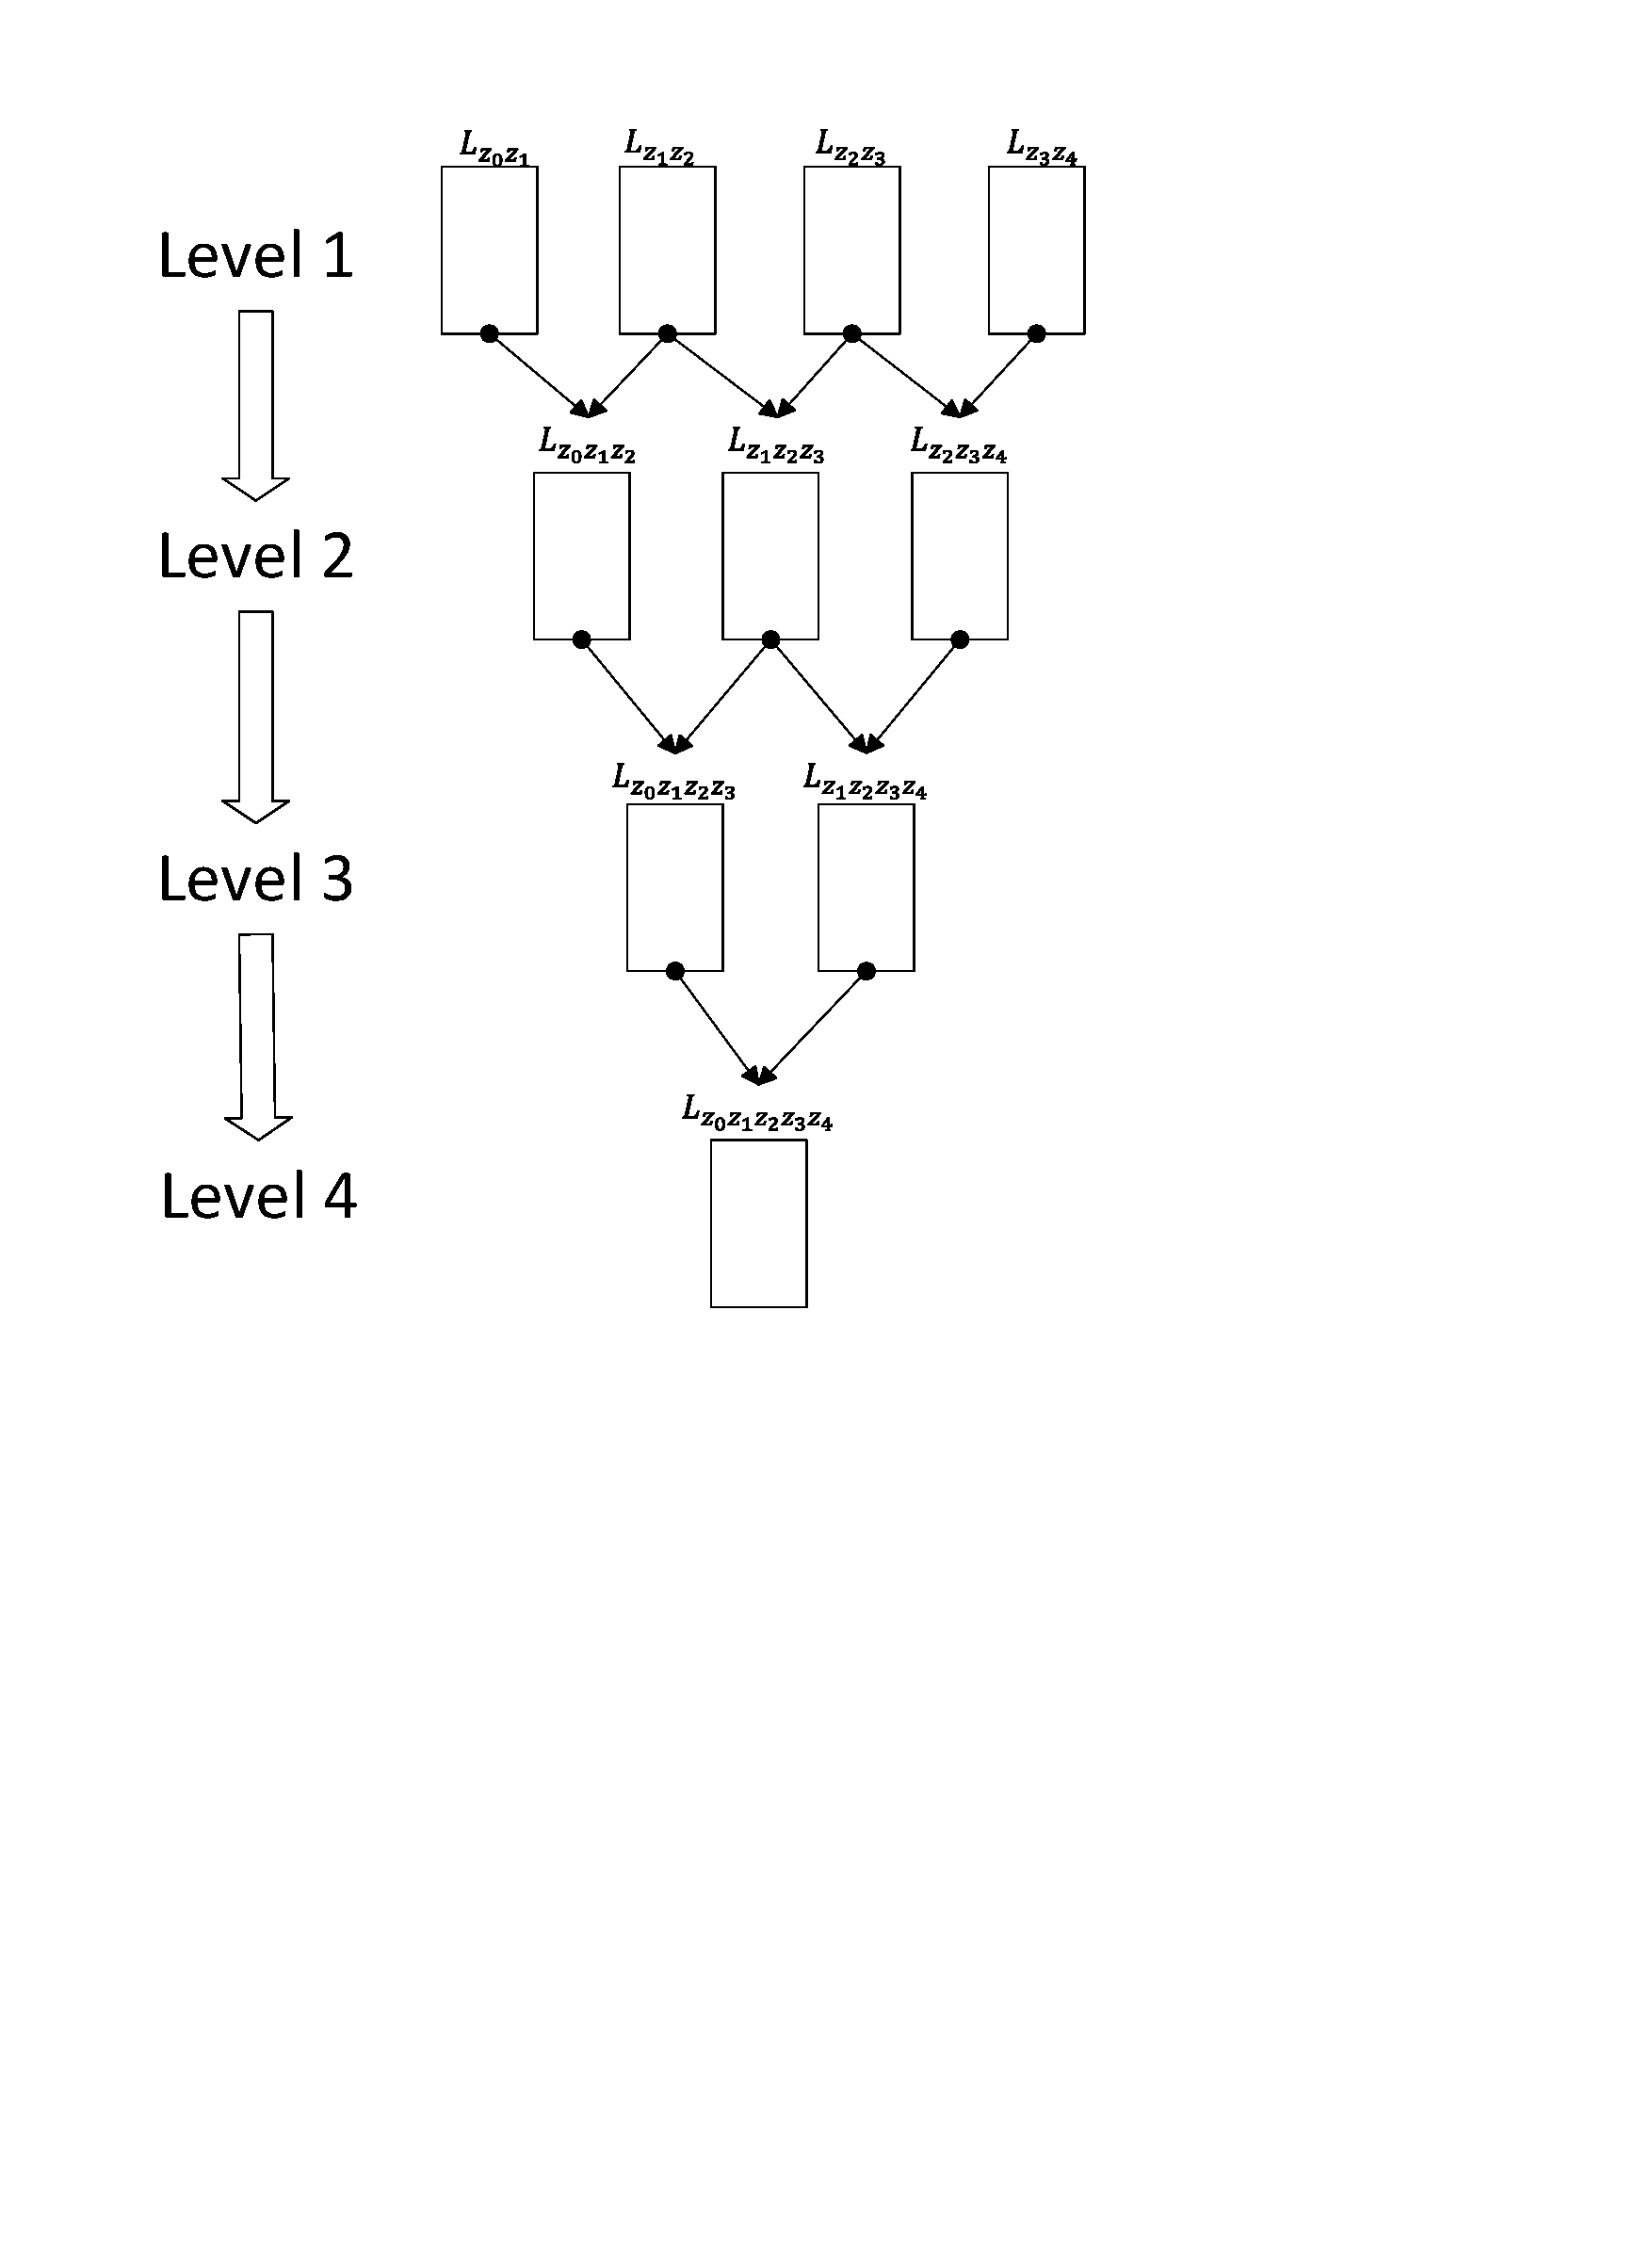
\includegraphics[width=0.5\textwidth]{pic/MergeZhang.pdf}
  \caption{The general process of Zhang's attack in \cite{AC:Zhang19}}\label{fig:MergeZhang}
\end{figure}

The most crucial step in Zhang \etal's attack in \cite{AC:Zhang19} is the recovery of the 33-bit CP based on the first 5 keystream bits $z_0,\ldots, z_4$.
Such a CP-recovery step can be summarized as the list-merging process in Fig. \ref{fig:MergeZhang}.
In Fig. \ref{fig:MergeZhang}, the list $L_{z_i\ldots z_j}$ ($i<j$) contains the state $\vec{s}^i$'s whose state bits are only partially known:
for each $\vec{s}^i\in L_{z_i\ldots z_j}$, the known bits are at positions $\lambda\subseteq [0,63]$ \st the knowledge of $\vec{s}^i[\lambda]$ can produce the consecutive output bits $z_i,\ldots, z_j$ following the A5/1 keystream generation process.
Specifically, for a list $L_{z_iz_{i+1}}$ at Level 1, 2 consecutive keystream bits $z_iz_{i+1}$ can be related to at most 15 state bits at positions $\lambda_0$ in \eqref{eq:KnownBitsL1}.
\begin{equation}\label{eq:KnownBitsL1}
\lambda_0=\{7,8,16,17,18,  28,29,38,39,40,  50,51,61,62,63\}
\end{equation}
The number of known state bits for 3, 4 and 5 consecutive keystream bits will grow to at most 21, 27 and 33 respectively.
Therefore, finally at Level 4, it is claimed by Zhang \etal in \cite{AC:Zhang19} each element $\vec{s}^0\in L_{z_0z_1z_2z_3}$ should contain 33 bits.
When merging two lists at the same level, the known bits at the overlapped positions are to be used as filters: only the elements share the same value at the overlapped positions can be merged as an element in the list in the next level.
Since each element in the lists contains at most 33 known bits, \cite{AC:Zhang19} claims that the elements in all lists can be stored with 5 bytes of memory.
However, Zhang \etal has never fully implement the process in Fig. \ref{fig:MergeZhang}:
they only implement the process from Level 1 to 2.
Without detailed analysis, Zhang \etal simply claim that the whole list merging process can be finished with a time complexity $2^{28.3}$ cipher ticks and the final list $L_{z_0z_1z_2z_3z_4}$ only contains $2^{16.6}$ elements.

Another feature of Zhang \etal's attack is the construction of the 4 initial lists: they employ the idea of near collision to construct the lists $L_{z_0z_1},\ldots, L_{z_3z_4}$.
They consider the low-hamming-weight internal state difference (ISD) $\Delta \vec{s}$ as follows:
\begin{equation}\label{eq:LowWeightISD}
  \mathcal{D}_2:=\left\{\Delta\vec{s}| hw(\Delta\vec{s})\leq 2 \text{ and } \Delta\vec{s}[i]=0  \text{ for all } i\notin\lambda_1 \right\}
\end{equation}
Apparently, there are $\binom{15}{0}+\binom{15}{1}+\binom{15}{2}=121$ elements in the ISD set $\mathcal{D}_2$ in \eqref{eq:LowWeightISD}.
But Zhang \etal find that only 99 ISDs $\mathcal{D}_2$ can result in the 2-bit output difference ${\tt 0x3}$.
Therefore, they store such 99 low-hamming-weight ISD's in a table $\mathcal{T}$ defined in \eqref{eq:99LowWeightISD}.
\begin{equation}\label{eq:99LowWeightISD}
  \mathcal{T}:=\left\{\Delta\vec{s}\in \mathcal{D}_2|
  \exists \vec{s}^0 \Rightarrow z_0z_1(\vec{s}^0)\oplus z_0z_1(\vec{s}^0\oplus \Delta\vec{s}) ={\tt 0x3}
  \right\}
\end{equation}
For a static 2-bit output $z_0z_1$,
Zhang \etal propose Algorithm \ref{alg:getLz0z1} to generate list of states $L_{z_0z_1}$, making sure that all elements in the list can result in  $z_0z_1$ directly.
In Zhang \etal's attack, they set the number limit $T=4\cdot 2^{15}/99=1323$ which results in the output list size 7963 and the correct state can be covered by $L_{z_0z_1}$ with probability $p_1=0.9835$.
In order to improve the probability that the list contains the correct state, Zhang \etal further propose the distilling process.
For positive integers $\eta$ and $\zeta$, the distilling process first generate $\eta\times \zeta$ lists with Algorithm \ref{alg:getLz0z1}; then, intersection and union operations are carried out as \eqref{eq:Distilling}.
\begin{equation}\label{eq:Distilling}
 L_{z_0z_1} \leftarrow U(\eta, \zeta)=
  \bigcup_{i=1}^{\eta}\left(\bigcap_{j=1}^\zeta L^{i,j}_{z_0z_1}\right)
  \text{ where }
  L^{i,j}_{z_0z_1}\leftarrow
  {\tt getList}(z_0z_1, T)
\end{equation}
According to Zhang \etal, when $\eta=2, \zeta=6$, the correct state can be covered by $L_{z_0z_1}$ with probability 0.9903.

\begin{algorithm}[htbp]
	\caption{Generate the internal states resulting in the given 2-bit output} \label{alg:getLz0z1}
	\begin{algorithmic}[1]
		\Procedure{{\tt getList}}{output bits $z_0z_1\in \mathbb{F}_2^2$, the number limit $T$}
\State Initialize an empty list $L_{z_0z_1}\leftarrow \phi$
\State Declare $\hat{z}_0\hat{z}_1\leftarrow z_0z_1\oplus {\tt 0x3}$
\State Generate $T$ states $\vec{\hat{s}}^0$ that only have non-zero elements at positions $\lambda_1$ and can result in the output $\hat{z}_0\hat{z}_1$
\For{$\Delta \vec{s}\in \mathcal{T}$}
\State Construct state $\vec{s}^0$
\If{$\vec{s}^0$ can result in the output $z_0z_1$}
\State Update $L_{z_0z_1}\leftarrow L_{z_0z_1}\cup \{\vec{s}^0\}$
\EndIf
\EndFor
\State \textbf{Return} $L_{z_0z_1}$
		\EndProcedure
	\end{algorithmic}
\end{algorithm}



After the CP-recovery phase, the adversary has already acquire $2^{16.6}$ $\vec{s}^0$'s in $L_{z_0z_1z_2z_3}$.
For each such $\vec{s}^0$, the corresponding $\vec{s}^5$ can be directly with the knowledge of 33 bits in CP.
For RP-recovery, Zhang \etal guess the $3y$ clock bits in \eqref{eq:RpGuessZhang} and construct linear equations of unknown RP bits according both guesses and output bits $z_5,\ldots, z_{5+y-1}$.
\begin{equation}\label{eq:RpGuessZhang}
  \vec{s}^5[8,29,51], \ldots, \vec {s}^{5+y-1}[8,29,51]
\end{equation}
They claim that the RP bits can be recovered with complexity approximately $2^{30}$ which is also the overall time complexity of the whole attack.
But there is no further details on how the different $y$'s can affect the complexities. 
It is unknown how effective the linear equation system can be in filtering wrong states. 
It is also unknown which $y$ should be used to identify the uniquely correct internal state $\vec{s}^0$.
 
We are to prove that almost all Zhang \etal's claims above are wrong in Section \ref{sec:ZhangWrongCompAnalysis}.
The analysis of $y$-effects are to be analyzed in detail in Section \ref{sec:ZhangRpRecovery} only to find that their complexity analysis is far too optimistic to be true.

\section{Move Patterns and Their Bit Condition Representations}\label{sec:MovePatternAndBC}
For each step $t=0,1,2\ldots$, whether the registers $\vec{R1},\vec{R2},\vec{R3}$ are updated or not depends on the three control bits $\vec{s}^t[8,29,51]$. %$(\vec{r_1^t}[8],\vec{r_2^t}[10],\vec{r_3^t}[10])$.
For all $2^3$ $\vec{s}^t[8,29,51]$ values, there are 4 possible move patterns denoted as Move 0, 1, 2 and 3.
Each movement corresponds to 2 $(\vec{r_1^t}[8],\vec{r_2^t}[10],\vec{r_3^t}[10])$ values and can also be represented as linear equations of state bits, which are also referred as the bit conditions.
Move 0-4 and their bit conditions are defined as follows:
\begin{description}
  \item[Move 0] $\tt{updateR1}$ in \eqref{eq:UpdateR1}, $\tt{updateR2}$ in \eqref{eq:UpdateR2} and $\tt{updateR3}$ in \eqref{eq:UpdateR3} are all called.
  The $\vec{s}^t[8,29,51]$ values are $(0,0,0)$ and $(1,1,1)$.
  The bit conditions are:
  \begin{equation}\label{eq:Move0BitCondition}
        \left\{
    \begin{aligned}
    &\vec{s}^t[8]\oplus \vec{s}^t[29]=0\\
    &\vec{s}^t[8]\oplus \vec{s}^t[51]=0
    \end{aligned}
    \right.
    \Leftrightarrow
    \left\{
    \begin{aligned}
    &\vec{R1}^t[8]=\vec{R2}^t[10]\\
    &\vec{R1}^t[8]=\vec{R3}^t[10]
    \end{aligned}
    \right.
  \end{equation}
  \item[Move 1] Only $\tt{updateR2}$ and $\tt{updateR3}$ are called.
  The $\vec{s}^t[8,29,51]$ values are $(0,1,1)$ and $(1,0,0)$.
  The bit conditions are:
  \begin{equation}\label{eq:Move1BitCondition}
    \left\{
    \begin{aligned}
    &\vec{s}^t[8] \oplus \vec{s}^t[29]=1\\
    &\vec{s}^t[8] \oplus \vec{s}^t[51]=1
    \end{aligned}
    \right.
    \Leftrightarrow
    \left\{
    \begin{aligned}
    &\vec{R1}^t[8]=\vec{R2}^t[10]\oplus 1\\
    &\vec{R1}^t[8]=\vec{R3}^t[10]\oplus 1
    \end{aligned}
    \right.
  \end{equation}
  \item[Move 2] Only $\tt{updateR1}$ and $\tt{updateR3}$ are called.
  The $\vec{s}^t[8,29,51]$ values are $(1,0,1)$ and $(0,1,0)$.
  The bit conditions are:
  \begin{equation}\label{eq:Move2BitCondition}
    \left\{
    \begin{aligned}
    &\vec{s}^t[8]\oplus \vec{s}^t[29]=1\\
    &\vec{s}^t[8]\oplus \vec{s}^t[51]=0
    \end{aligned}
    \right.
    \Leftrightarrow
    \left\{
    \begin{aligned}
    &\vec{R1}^t[8]=\vec{R2}^t[10]\oplus 1\\
    &\vec{R1}^t[8]=\vec{R3}^t[10]
    \end{aligned}
    \right.
  \end{equation}
  \item[Move 3] Only $\tt{updateR1}$ and $\tt{updateR2}$ are called.
  The $\vec{s}^t[8,29,51]$ values are $(1,1,0)$ and $(0,0,1)$.
  The bit conditions are:
  \begin{equation}\label{eq:Move3BitCondition}
    \left\{
    \begin{aligned}
    &\vec{s}^t[8]\oplus \vec{s}^t[29]=0\\
    &\vec{s}^t[8]\oplus \vec{s}^t[51]=1
    \end{aligned}
    \right.
    \Leftrightarrow
    \left\{
    \begin{aligned}
    &\vec{R1}^t[8]=\vec{R2}^t[10]\\
    &\vec{R1}^t[8]=\vec{R3}^t[10]\oplus 1
    \end{aligned}
    \right.
  \end{equation}
\end{description}
We denote the movement $\vec{s}^t\rightarrow \vec{s}^{t+1}$ as $m^t\in \mathbb{F}_2^2= \{0,1,2,3\}$.
So the movements corresponding to the output keystream bits $z^0,\ldots, z^t$ are $m^0,\ldots, m^t$.
In our guess and determine attack, we first guess the movement $m^t$ corresponding to $\vec{s}^t\rightarrow \vec{s}^{t+1}$ and maintains a bit condition set $\mathcal{BC}$ by adding new bit conditions corresponding to the new movement $m^t$ and the output $z^t$.
For each step $t$, there are 3 bit conditions: 2 are from one of \eqref{eq:Move0BitCondition}, \eqref{eq:Move1BitCondition}, \eqref{eq:Move2BitCondition}, \eqref{eq:Move3BitCondition} according to the move guess and the rest is from the output $z^t$ as
\begin{equation}\label{eq:OutputBitCondition}
\vec{s}^{t+1}[18]\oplus \vec{s}^{t+1}[40]\oplus \vec{s}^{t+1}[63]=z^t
\end{equation}
So each move guess can deduce 3 bit conditions.
In Section \ref{sec:OurGuessAndDetermine}, we guess the moves $m^0,\ldots, m^{t-1}$ and maintain a bit condition system to distinguish the correct state $\vec{s}^0$ from the wrong ones.


\section{Move Guessing v.s. Clock Guessing}\label{sec:MoveVsClockGuess}
Our move guessing method differs from the previous guessing strategies.
In \cite{AC:Zhang19} as well as all previous A5/1 cryptanalysis papers, the adversary guesses directly the 3 clock bits $\vec{s}^t[8,29,51]$ rather than the 2-bit move $m^t$.
Apparently, our 2 move bits can be deduced from the 3 clock bits.
Let $m^t[0,1]=(\mu, \nu)\in \mathbb{F}_2^2$ and the corresponding clock bits are $\vec{s}^t[8,29,51]=(\rho,\varrho, \sigma)\in \mathbb{F}_2^3$, the two bits $(\mu, \nu)$ can be deduced from $(\rho,\varrho, \sigma)$ as \eqref{eq:MoveAndClockBitRelation}
\begin{equation}\label{eq:MoveAndClockBitRelation}
\begin{aligned}
  \mu=\bar{\rho}\bar{\varrho}\sigma \oplus
  \bar{\rho}\varrho \sigma \oplus
  \rho \bar{\varrho} \bar{\sigma} \oplus
  \rho \varrho \bar{\sigma} \\
  \nu=\bar{\rho}\bar{\varrho}\sigma \oplus
  \bar{\rho}\varrho\bar{\sigma} \oplus
  \rho\bar{\varrho}\sigma \oplus
  \rho \varrho \bar{\sigma}
\end{aligned}
\end{equation}
where $\bar{x}$ is the NOT operation equivalent to $x\oplus 1$.
From the bit condition point of view, a 3-bit guess  $\vec{s}^t[8,29,51]=(\rho,\varrho, \sigma)$ is naturally 3 bit conditions.
The 3 bit conditions are also equivalent to 2 move-oriented  bit conditions and a bit value condition $\vec{s}^t[8]=\rho$.
For example, if the clock bit values are of the form $\vec{s}^t[8,29,51]=(\rho, \rho, \rho)$, which corresponds to the Move 0, the 3 bit conditions can also be regarded as adding $\vec{s}^t[8]=\rho$ to the Move 0 constraints in \eqref{eq:Move0BitCondition} as shown in \eqref{eq:ClockMove0Equiv}.
\begin{equation}\label{eq:ClockMove0Equiv}
  \left\{
  \begin{aligned}
    &\vec{s}^t[8]=\rho\\
    &\vec{s}^t[29]=\rho\\
    &\vec{s}^t[51]=\rho
  \end{aligned}
  \right.
  \Leftrightarrow
  \left\{
    \begin{aligned}
  &\vec{s}^t[8]=\rho\\
  &\left\{
  \begin{aligned}
    &\vec{s}^t[8]\oplus\vec{s}^t[29]=0\\
    &\vec{s}^t[8]\oplus\vec{s}^t[51]=0
  \end{aligned}
  \right.
    \end{aligned}
  \right.
\end{equation}
Such an equivalence is also true for other clock bit values and move patterns.
Adding the bit condition of the output in \eqref{eq:OutputBitCondition}, we know that each 3-bit guess of the clock bits $\vec{s}^t[8,29,51]$ can deduce 4 bit conditions while each of our 2-bit guess of $m^t$ can deduce 3 bit conditions.
On average, our move guessing method seems more efficient because each move guess can result in 1.5 bit conditions while the number of bit condition for each clock bit guess is no more than 1.34.
But it remains to be checked whether the clock-oriented bit conditions can also be better filters for eliminating wrong internal states.
To make fair comparison between the two strategies, we apply both move and clock guessing strategy in the RP-recovery phase of Zhang \etal's attack in \cite{AC:Zhang19}.
The results show that move guessing can result in slightly lower complexities than its clock counterpart.
Details can be seen later in Section \ref{sec:OurRpRecovery} and \ref{sec:ZhangRpRecovery}.

\section{Our State-Recovery Attack based on the Move Guessing Strategy}\label{sec:OurGuessAndDetermine}
As can be seen, the move conditions \eqref{eq:Move0BitCondition}, \eqref{eq:Move1BitCondition}, \eqref{eq:Move2BitCondition}, \eqref{eq:Move3BitCondition} and the output condition \eqref{eq:OutputBitCondition} correspond to the internal state at different time instances.
But our attack is targeted to recovering the initial state $\vec{s}^0$.
Therefore, we need to represent the internal states at different time instance $t$ with $\vec{s}^0$ so that the bit conditions are represented by $\vec{s}^0$ bits as well.
With the knowledge of $m^0,\ldots, m^{t-1}$, $\vec{s}^{t}$ can be iteratively deduced from $\vec{s}^{0}$ and each $\vec{s}^{t}$ bit can be expressed as a linear combination of $\vec{s}^0$ bits.
Since a linear combination of $\vec{s}^0$ bits can also be regarded as a inner-product of $\vec{s}^0$ and a 64-bit word $\vec w\in \mathbb{F}_2^{64}$, we can track each $\vec{s}^0,\ldots, \vec{s}^t$ bits with 64 64-bit words denoted as $W^0,\ldots, W^t\in (\mathbb{F}_2^{64})^{64}$.
The initial $W^0$ corresponds to $\vec{s}^0$ is defined naturally as \eqref{eq:W0ofS0}
\begin{equation}\label{eq:W0ofS0}
  W^0=(\vec e_0, \ldots, \vec e_{63}), \text{ where } \vec e_i[j]=\left\{
  \begin{split}
     1 &\quad i=j \\
     0 &\quad j\in [0,63]\backslash\{i\}
  \end{split}
  \right.\text{ for }i=0,\ldots, 63
\end{equation}
so as to make sure $W^0[i]\cdot \vec{s^0}=\vec{e}_i\cdot \vec{s}^0=\vec{s}^0[i]$ for $i=0,\ldots, 63$.
With $W^0,\ldots, W^{t-1}$, the word vector $W^{t}$ can be deduced from $W^{t-1}$ according to the movement $m^{t=1}$ by calling
$W^{t}\leftarrow {\tt UpdW}(m^{t-1}, W^{t-1})$ described in Algorithm \ref{alg:updateW}.
With the knowledge of $W^t$, each state bit of $\vec{s}^t$ can be uniformly expressed as a linear combination of $\vec{s}^0$ bits as
\begin{equation}\label{eq:ExpressStwithS0}
\vec{s}^t[i]=W^t[i]\cdot \vec{s}^0
\end{equation}
For $t$ consecutive movements $m^0,\ldots,m^{t-1}$ and the corresponding output $z^0,\ldots, z^{t-1}$, we can deduce the corresponding bit condition set $\mathcal{BC}$ as $\mathcal{BC}\leftarrow {\tt{getBC}}((m^0,\ldots, m^{t-1}), (z^0,\ldots, z^{t-1}))$ where ${\tt{getBC}}$ is defined as Algorithm \ref{alg:getBC}.
The bit condition set $\mathcal{BC}$ can be regarded as a linear equation system in \eqref{eq:BCLpSystem}
\begin{equation}\label{eq:BCLpSystem}
  A\vec x^T=\vec b^T, \text{ where } A\in \mathbb{F}_2^{3t\times 64}, \vec x\in \mathbb{F}_2^{64}, \vec b\in \mathbb{F}_2^{3t}
\end{equation}
and the solutions to the linear system in \eqref{eq:BCLpSystem} is exactly the possible values of the internal state $\vec{s}^0$'s resulting in the output keystream bits $z_0,\ldots, z_{t-1}$.
The number of solutions to \eqref{eq:BCLpSystem} depends on the order of the matrix $A$ and its extended matrix
\begin{equation}\label{eq:ExtendedMatrixOfA}
  E=[A,\vec b^T]
\end{equation}
If $order(A)=order(E)$, there will be $2^{64-order(A)}$ solutions; otherwise, there will be no solutions at all.
Apparently, the matrix $A$ and the vector $\vec b$ are both deduced according to the move guesses $m^0,\ldots, m^{t-1}$ and the output bits $z^0,\ldots, z^{t-1}$.
For the correct guess of $m^0,\ldots, m^{t-1}$, the relation $order(A)=order(E)$ holds constantly; for the wrong guesses, however, there should be a probability $1-\alpha_t$ ($0\geq \alpha_t\leq 1$) that $order(A)\neq order(E)$.
Based on such a finding, the general process of our state-recovery attack can be divided naturally into 3 main steps:
\begin{description}
  \item[S1] Guess moves $m^0,\ldots, m^{t-1}$ and maintain a bit-condition-based linear system in \eqref{eq:BCLpSystem}
  \item[S2] Do the matrix order test and discard the wrong guesses satisfying  $order(A)\neq order(E)$
  \item[S3] Deduce the remaining $\vec{s}^0$ candidates and identify the correct $\vec{s}^0$ with additional output bits $z^{t},\ldots, z^{\ell-1}$ generated by the encryption oracle
\end{description}
Therefore, the detailed description of our move-guessing-based state-recovery attack is as follows:
\begin{enumerate}
  \item Query the A5/1 encryption oracle for $\ell$ keystream bits $z^0,\ldots, z^{\ell-1}$
  \item Initialize an empty set $\mathcal{S}$ of $\vec{s}^0$ candidates
  \item For some $t<\ell$, we guess the $2^{2t}$ movements $(m^0,\ldots, m^{t-1})$, acquire the bit conditions $\mathcal{BC}\leftarrow {\tt getBC}((m^0,\ldots, m^{t-1}), (z^0,\ldots, z^{t-1}))$ by calling Algorithm \ref{alg:getBC} (\textbf{S1}) and do the following substeps:
      \begin{enumerate}
        \item Deduce the $A$ and $\vec b$ in \eqref{eq:BCLpSystem} according to $\mathcal{BC}$ and compute the extended matrix $E$ in \eqref{eq:ExtendedMatrixOfA}
        \item Compute $order(A)$ and $order(E)$, if $order(A)\neq order(E)$, such a movement guess is wrong, go back to Step 2 for the next movement guess (\textbf{S2})
        \item For all $2^{64-order(A)}$ solutions to $A\vec x^T=b^T$, set $\vec{\hat{s}}^0\leftarrow \vec x$ and generate the keystream bits $\hat{z}^0,\ldots, \hat{z}^{t-1},\hat{z}^{t},\ldots, \hat{z}^{\ell-1}$
        \item If $(\hat{z}^{t},\ldots, \hat{z}^{\ell-1})=(z^{t},\ldots, z^{\ell-1})$, add such $\vec{\hat{s}}^0$ into $\mathcal{S}$ (\textbf{S3})
      \end{enumerate}
  \item Return $\mathcal{S}$
\end{enumerate}
When $\ell$ is large enough, there should be only 1 element in $\mathcal{S}$ which is exactly the correct internal state $\vec{s}^0$.

\noindent\textbf{Complexity Analysis. }
In Step 3, there are $2^{2t}$ candidate moves $(m^0,\ldots, m^{t-1})$ and not all of them can pass the $order(A)=order(E)$ test Step 3.(b).
We suppose that there is an positive number $0\leq \alpha_t \leq 1$ that averaging $\alpha_t  2^{2t}$ candidate moves can pass the test.
We further denote the averaging $order(A)$ as $\beta_t $.
With $\alpha_t ,\beta_t $, the averaging time complexity can be computed as follow:
\begin{equation}\label{eq:Complexity}
  Comp=2^{2t}+\alpha_t \cdot 2^{2t+64-\beta_t }=2^{2t}+2^{2t+64-\beta_t +\log\alpha_t }
\end{equation}
We randomly select $2^{30}$ $((m^0,\ldots, m^{t-1}), (z^0,\ldots, z^{t-1}))$ pairs and do the 3.(b) test to compute the averaging $\alpha_t$ and $\beta_t$ for $t$'s.
We find that when $t<14$, $\alpha_t$ are larger than 0.5 ($\log\alpha_t\geq -1$) and $\beta_t\leq 3t$ so the overall complexity is constantly larger than $2^{50}$.
For $14\leq t\leq 29$, the $\alpha_t$, $\beta_t$ and $Comp$ are listed in Table \ref{tab:AlphaAndBeta}.
As can be seen, the lowest time complexity appears at $t=21$ with $Comp=2^{43.91}$.
As can be seen in Table \ref{tab:AlphaAndBeta}, the order $\beta_t$ has already climbed to almost 64 for $t=27$.
So we can safely set $\ell=32$ to filter the wrong move guesses.
According to our experiment, $\ell=32$ is well enough to identify the correct $\vec{s}^0$ so the data complexity of our attack is only 32 bits.
The memory complexity is only $\mathcal{BC}$ and the corresponding matrix $A$ as well as its extended matrix $E$ in \eqref{eq:BCLpSystem} and \eqref{eq:ExtendedMatrixOfA}.
The memory complexity is only $O(t)$ and, to be more specific, $2\cdot (64+1)\cdot 3t\leq 12480$ bits which is bounded by 2KB.
So the memory complexity is practical and negligible in comparison with previous attacks.

\begin{table}[htbp]
  \centering
  \caption{The averaging $\alpha_t$ and $\beta_t$ in \eqref{eq:Complexity} with $2^{30}$ random tests}\label{tab:AlphaAndBeta}
    \begin{tabular}{|l|l|l|l|l|l|l|l|}
    \hline
    \multicolumn{1}{|c|}{$t$} & \multicolumn{1}{c|}{$\beta_t$} & \multicolumn{1}{c|}{$\log\alpha_t$} & \multicolumn{1}{c|}{$\log Comp$} & \multicolumn{1}{c|}{$t$} & \multicolumn{1}{c|}{$\beta_t$} & \multicolumn{1}{c|}{$\log\alpha_t$} & \multicolumn{1}{c|}{$\log Comp$} \\
    \hline

    14    & 41.959 & -0.028 & 50.013 & 22    & 61.604 & -3.971 & 44.417 \\
    \hline
    15    & 44.868 & -0.095 & 49.037 & 23    & 62.781 & -5.915 & 46.055 \\
    \hline
    16    & 47.683 & -0.231 & 48.085 & 24    & 63.433 & -8.420 & 48.006 \\
    \hline
    17    & 50.381 & -0.468 & 47.151 & 25    & 63.755 & -11.173 & 50.001 \\
    \hline
    18    & 52.955 & -0.813 & 46.233 & 26    & 63.904 & -14.060 & 52.000 \\
    \hline
    19    & 55.409 & -1.270 & 45.330 & 27    & 63.967 & -17.027 & 54.000 \\
    \hline
    20    & 57.734 & -1.852 & 44.481 & 28    & 63.990 & -20.021 & 56.000 \\
    \hline
    21    & 59.860 & -2.671 & \textbf{43.914} & 29    & 63.997 & -23.117 & 58.000 \\
    \hline

    \end{tabular}%
\end{table}%


\begin{algorithm}[htbp]
	\caption{Deduce the equation word set according to a movement} \label{alg:updateW}
	\begin{algorithmic}[1]
		\Procedure{{\tt UpdW}}{movement $m^t\in \{0,3\}$, words $W^t\in (\mathbb{F}_2^{64})^{64}$}
\If{$m^t=0$}
\State $A^t\leftarrow {\tt{UpdWR}}(W^t,1)$
\State $B^t\leftarrow {\tt{UpdWR}}(A^t,2)$
\State $W^{t+1}\leftarrow {\tt{UpdWR}}(B^t,3)$
\EndIf
\If{$m^t=1$}
\State $B^t\leftarrow {\tt{UpdWR}}(W^t,2)$
\State $W^{t+1}\leftarrow {\tt{UpdWR}}(B^t,3)$
\EndIf
\If{$m^t=2$}
\State $A^t\leftarrow {\tt{UpdWR}}(W^t,1)$
\State $W^{t+1}\leftarrow {\tt{UpdWR}}(A^t,3)$
\EndIf
\If{$m^t=3$}
\State $A^t\leftarrow {\tt{UpdWR}}(W^t,1)$
\State $W^{t+1}\leftarrow {\tt{UpdWR}}(A^t,2)$
\EndIf
\State \textbf{Return } $W^{t+1}$
		\EndProcedure
	\end{algorithmic}
\begin{algorithmic}[1]
		\Procedure{{\tt UpdWR}}{words $W\in (\mathbb{F}_2^{64})^{64}$, register number $n\in \{1,2,3\}$}
\State Initialize $X\in (\mathbb{F}_2^{64})^{64}$ as $X\leftarrow W$
\If{$n=1$}
\For{$i=1,\ldots,18$}
\State Update the $i$-th entry of $X$ as $X[i]\leftarrow W[i-1]$
\EndFor
\State Compute the 0-th entry of $X$ as $X[0]\leftarrow W[18]\oplus W[17]\oplus W[16]\oplus W[13]$ according to \eqref{eq:UpdateR1}
\EndIf
\If{$n=2$}
\For{$i=20,\ldots,40$}
\State Update the $i$-th entry of $X$ as $X[i]\leftarrow W[i-1]$
\EndFor
\State Compute the 19-th entry of $X$ as $X[19]\leftarrow W[40]\oplus W[39]$ according to \eqref{eq:UpdateR2}
\EndIf
\If{$n=3$}
\For{$i=42,\ldots,63$}
\State Update the $i$-th entry of $X$ as $X[i]\leftarrow W[i-1]$
\EndFor
\State Compute the 41-th entry of $X$ as $X[19]\leftarrow W[63]\oplus W[62]\oplus W[61]\oplus W[48]$ according to \eqref{eq:UpdateR3}
\EndIf
\State \textbf{Return } $X$
		\EndProcedure
	\end{algorithmic}
\end{algorithm}

\begin{algorithm}[htbp]
	\caption{Deduce the set of bit conditions according to the given moves and output bits} \label{alg:getBC}
	\begin{algorithmic}[1]
		\Procedure{{\tt getBC}}{movements $(m^0,\ldots, m^{t-1})\in \{0,3\}^t$, output bits $(z^0,\ldots, z^{t-1})\in \mathbb{F}_2^{t}$}
\State Initialize the words $W^0\leftarrow (\vec e_0,\ldots, \vec e_{63})$ according to \eqref{eq:W0ofS0}
\State Initialize the bit condition set as empty: $\mathcal{BC}\leftarrow \phi$
\State Initialize $\vec{x}=(x_0,\ldots, x_{63})$ as vector of 63 unknown boolean variables corresponding to the 64 state bits of $\vec s^0$
\For{$i=0,1,\ldots, t-1$}
\If{$m^i=0,1,2,3$}
\State Update $\mathcal{BC}$ by adding the following conditions corresponding to \eqref{eq:Move0BitCondition}, \eqref{eq:Move1BitCondition}, \eqref{eq:Move2BitCondition}, \eqref{eq:Move3BitCondition}:
\[
\left\{
\begin{aligned}
(W^i[8]\oplus W^i[29])\cdot \vec x&=\delta(m^i)\\
(W^i[8]\oplus W^i[51])\cdot \vec x&=\varrho(m^i)
\end{aligned}
\right.
\]
where $(\delta(m^i), \varrho(m^i))=(0,0),(1,1),(1,0),(0,1)$ for $m_i=0,1,2,3$ respectively
\EndIf
\State Deduce $W^{i+1}$ according to $W^{i}$ by calling $W^{i+1}\leftarrow {\tt UpdW}(m^i,W^i)$ defined in Algorithm \ref{alg:updateW}
\State Update $\mathcal{BC}$ by adding the following bit condition corresponding to \eqref{eq:OutputBitCondition}
\[
(W^{i+1}[18]\oplus W^{i+1}[40]\oplus W^{i+1}[63])\cdot \vec x =z^i
\]
\EndFor
\State \textbf{Return} $\mathcal{BC}$
		\EndProcedure
	\end{algorithmic}
\end{algorithm}


\section{Revisit Zhang's Attack in \cite{AC:Zhang19}}
As has been briefly mentioned in Section \ref{sec:BriefReviewZhangAttack}, Zhang \etal has never fully implemented their attack in \cite{AC:Zhang19}:
they only implement the 1st step of the CP-recovery phase, which is Level 1 to 2 in Fig. \ref{fig:MergeZhang}.
The details of the following CP-recovery steps and the whole RP-recovery phase are absent, leaving it unknown whether the whole attack can work as claimed.

To verify their attack, we fully implement their attack only to find several mistakes and the complexity evaluation to the whole attack is far too optimistic.
Section \ref{sec:ZhangWrongP1} and \ref{sec:ZhangWrongCompAnalysis} gives the wrong evaluations of several crucial parameters in \cite{AC:Zhang19}.
Section \ref{sec:ZhangRpRecovery} supplements Zhang \etal's attack with all the missing details in the CP- and RP-recovery phases and gives a correct complexity evaluation to the original attack in \cite{AC:Zhang19}.
Section \ref{sec:OurRpRecovery} replaces Zhang \etal's clock-guess-based RP-recovery with our move-guess-based one to show the advantage of our technique.

\subsection{Zhang's Wrong Evaluation to $p_1$ and the Success Probability}\label{sec:ZhangWrongP1}
In \cite{AC:Zhang19}, Zhang \etal claim that, for $T=4\cdot 2^{15}/99$, a randomly constructed list $L_{z_0z_1}\leftarrow {\tt getList}(z_0z_1, T)$ acquired by calling Algorithm \ref{alg:getLz0z1} is of size 7963  and the correct internal state lies in $L_{z_0z_1}$ with probability $0.9835$.
However, we repeat the experiment $10^6$ times and the correct state lies in $L_{z_0z_1}$ for only 972436 times.
So it is safe for us to claim that the actual $p_1$ is $0.9725$: Zhang's evaluation in \cite{AC:Zhang19} is far too optimistic.
The reason why Zhang \etal made such a mistake is unknown.
Maybe their using RC4 as the source of randomness is not so qualified.
Our experiments have tried various random generators including Snow-V, AES, the NSF standard random number generator etc.
All these experiments reveal that the actual $p_1$ is 0.9725 rather than 0.9835: Zhang's evaluation in \cite{AC:Zhang19} is wrong.

With the corrected $p_1$, the probability for a distilled list $U$ in \eqref{eq:Distilling} to cover the correct state  should be reevaluated.
The corrected evaluation and as well as shown in Table \ref{tab:ProbInU}.
We read the source code\footnote{\url{https://github.com/martinzhangbin}} corresponding to \cite{AC:Zhang19} carefully only to find that the $|U|$ parameter is wrong because of wrong implementation:
when they try to get $(\eta , \zeta)$, they actually do $\zeta$ intersect operations so they actually acquire the $U(\eta,\zeta+1)$ instead.
As a consequence, the size $|U|$'s are smaller than expected.
Since the attack can only succeed when the correct internal state lies in $U$, so the parameter ${\tt Prob.}$ in Table \ref{tab:ProbInU} is actually the success probability to the whole attack.
Therefore, the success probability of Zhang's attack is far too optimistic as well.
\begin{table}[htbp]
  \centering
  \caption{Our evaluation (left) v.s. Zhang \etal's (right, quoted from \cite{AC:Zhang19})}
  \begin{minipage}[t]{0.45\textwidth}
  \centering
     \begin{tabular}{c|c|c|c}
    \hline
    $\eta$ & $\zeta$ & $|U|$ & {\tt Prob.} \\
    \hline
    \hline
    2     & 3     & 8109  & 0.9935 \\
    2     & 4     & 8050  & 0.9887 \\
    2     & 5     & 8009  & 0.9830 \\
    2     & 6     & 7948  & 0.9761 \\
    \hline
    \end{tabular}%
  \end{minipage}
  \begin{minipage}[t]{0.45\textwidth}
    \centering
        \begin{tabular}{c|c|c|c}
    \hline
   $\eta$ & $\zeta$  & $|U|$ & {\tt Prob.} \\
    \hline
    \hline
    2     & 3     & 8065  & 0.9940 \\
    2     & 4     & 7989  & 0.9927 \\
    2     & 5     & 7934  & 0.9912 \\
    2     & 6     & 7835  & 0.9903 \\
    \hline
    \end{tabular}%
  \end{minipage}
  \label{tab:ProbInU}%
\end{table}%

\subsection{Zhang's Wrong Evaluation to the CP-Recovery Complexities}\label{sec:ZhangWrongCompAnalysis}
Although Zhang \etal has never fully implemented the CP-recovery phase of their attack in \cite{AC:Zhang19}, they still give the following claims:
\begin{description}
  \item[Claim 1] The whole merging process in Fig. \ref{fig:MergeZhang} requires $2^{28.3}$ cipher ticks.
  \item[Claim 2] The final $L_{z_0z_1z_2z_3z_4}$ contains $2^{16.6}$ candidates.
  \item[Claim 3] The elements in the lists require at most 5 bytes of memory.
  \item[Claim 4] Each candidate in $L_{z_0z_1z_2z_3z_4}$ have 33 known bits.
\end{description}
Our practical implementation of the full attack proves that all the claims above are wrong.


Since the merging of two lists $L_1,L_2$ requires $|L_1|\cdot |L_2|$ operations, it is impossible to get exact evaluation to the complexities without actually knowing the sizes of all the lists.
According to our implementation, the sizes of the lists are as follows:
\begin{equation}\label{eq:ListSizes}
  \begin{aligned}
  |L_{z_iz_{i+1}}| &\approx 2^{12.95},\quad \text{ for } i=0,1,2, 3 \\
  |L_{z_iz_{i+1}z_{i+2}}| & \approx 2^{16.70},  \quad \text{ for } i=0,1, 2\\
  |L_{z_iz_{i+1}z_{i+2}z_{i+3}}| & \approx 2^{20.46},  \quad \text{ for } i=0, 1\\
  |L_{z_0z_{1}z_{2}z_{3}z_{4}}| & \approx 2^{24.21}
  \end{aligned}
\end{equation}
Therefore, the complexity of the merging process is dominated by Level 3 to 4 which is approximately $2^{20.46\cdot 2}=2^{40.92}$: far beyond $2^{28.3}$.
Zhang \etal's Claim 1 is wrong.
The size of $L_{z_0z_1z_2z_3z_4}$ is $2^{24.21}> 2^{16.6}$.
So Zhang \etal's Claim 2 is also wrong.

The merging process in Fig. \ref{fig:MergeZhang} takes two lists denoted as $L_t$ and $L_{t+1}$.
$L_{t}$ contains the partial states of $\vec{ s}^t$ while $L_{t+1}$ consists of partial states of $\vec{s}^{t+1}$.
According to Section \ref{sec:MovePatternAndBC}, a $\vec{s}^t$ should take a move $m^t\in \{0,1,2,3\}$ before reaching $\vec{s}^{t+1}$ and that move $m^t$ is decided by the three clock bits $\vec{s}^t[8,29,51]$.
So the merging step $\tilde{L}_t\leftarrow {\tt merge}(L_t, L_{t+1})$ is as follows:
\begin{enumerate}
  \item Initialize the merged list as empty $\tilde{L}_t\leftarrow \phi$.
  \item For each $(\vec{s}^t,\vec{s}^{t+1})\in L_t\times L_{t+1}$, do the following steps:
  \begin{enumerate}
    \item Identify the positions of the known bits in $\vec{s}^t$ denoted as $\lambda_0\subseteq [0,63]$.
    \item Determine the move $m^t$ according to 3 known clock bits $\vec{s}^t[8,29,51]$.
    \item Determine the state $\vec{\hat{s}}^t$ \st $\vec{\hat{s}}^t\xrightarrow[]{m^t} \vec{s}^{t+1}$
    \item Identify the positions of the known bits in $\vec{\hat{s}^t}$ denoted as $\lambda_1\subseteq [0,63]$
    \item If $\vec{\hat{s}}^t[\lambda_0\cap \lambda_1]=\vec{s}^t[\lambda_0\cap \lambda_1]$, store the vector $\vec{\tilde{s}}^t\leftarrow \vec{\hat{s}}^t \vee \vec{s}^t$ in $\tilde{L}_t$ where $\vee$ is bitwise OR.
        The known bits of the newly generated  $\vec{\tilde{s}}^t$ is $\tilde{\lambda}\leftarrow\lambda_0\cup \lambda_1$.
  \end{enumerate}
  \item Return $\tilde{L}_t$
\end{enumerate}
According to the description above, any element $\vec{s}\in L$ should not only contain the value but the positions, denoted as $\lambda$, of the known bits as well.
At Level 1, since all list are generated through Algorithm \ref{alg:getLz0z1}, all elements share the same known-bit positions in \eqref{eq:KnownBitsL1}.
But the following Example \ref{examp:DifferentMoveKnownBits} shows that different moves will result in different known bit positions.
Example \ref{examp:DifferentMoveKnownBits} indicates that the known bits of the merged partial state $\vec{\tilde{s}}^t$ may not be exactly the 21 bits given in \cite{AC:Zhang19}: they are also likely to be subsets of the 21 bits.
\begin{example}\label{examp:DifferentMoveKnownBits}
  Let $(\vec{s}^0,\vec{s}^1)\in L_{z_0z_1}\times L_{z_1z_2}$.
  We have $\lambda_0=\lambda$ in \eqref{eq:KnownBitsL1}.
  If the move $m^0=0$ ($\vec{s}^0[8,29,51]\in\{(0,0,0),(1,1,1)\}$ according to \eqref{eq:MoveAndClockBitRelation} in Section \ref{sec:MoveVsClockGuess}), the known bit positions for $\vec{s}^1$ should be
  \[
  \lambda_1:=\{7-1,8-1,16-1,17-1,18-1,   28-1,29-1,38-1,39-1,40-1,  50-1,51-1,61-1,62-1,63-1  \}.
  \]
  and $\tilde{\lambda}=\lambda_0 \cup \lambda_1$ is of size $|\tilde{\lambda}|=21$.
  If the move is $m^0=1$ ($\vec{s}^0[8,29,51]\in  \{(1,0,0),(0,1,1)\}$), we have
  \[
  \lambda_1:=\{7,8,16,17,18,   28-1,29-1,38-1,39-1,40-1,  50-1,51-1,61-1,62-1,63-1  \}.
  \]
  and $|\tilde{\lambda}|=19$.
\end{example}
In order to keep merging the lists in Level 2-4, $\tilde{\lambda}$ containing the known bit positions should also be stored which takes the same size of the partial states.
Since the lists in Level 4 contain partial states of 33 bits, the $\tilde{\lambda}$'s are of the same size of 33 bits.
So the elements in the lists requires at most $\lceil 2\cdot 33/8\rceil=9$ bytes: Zhang \etal's Claim 3 is wrong.
Same with Example \ref{examp:DifferentMoveKnownBits}, the $\tilde{\lambda}$ for $\vec{\tilde{s}}^t\in L_{z_0z_1z_2z_3z_4}$ are more likely to be subsets of the 33 bits: Claim 4 of Zhang \etal is wrong.
In fact, according to our experiments, the number of known bits of $L_{z_0z_1z_2z_3z_4}$ elements are usually $|\tilde{\lambda}|\approx 30.14$, which is far below 33.
$|\tilde{\lambda}|$ can only be 33 when $m^0=\ldots= m^4=0$.
Such an event can happen with probability $2^{-10}$.


\subsection{Zhang \etal's Attack with The Original Clock-Guess-Based RP-Recovery}\label{sec:ZhangRpRecovery}
We have supplemented all the details of the list merging operations in Section \ref{sec:ZhangWrongCompAnalysis}.
The whole CP-recovery phase in Fig. \ref{fig:MergeZhang} can now be carried out.
At the end of CP-recovery, the adversary have got the list $L_{z_0z_1z_2z_3z_4}$.
Each $\vec{\tilde{s}}^0\in L_{z_0z_1z_2z_3z_4}$ corresponds to a set $\tilde{\lambda}\subseteq [0,63]$ containing the positions of known state bits and it guarantees that the first 5 keystream bits are exactly $z_0,\ldots, z_4$.
The known bits $\vec{\tilde{s}}^0[\tilde{\lambda}]$ can deduce directly the first 5 moves $m^0,\ldots, m^4$.
Therefore, the bit conditions for each $\vec{\tilde{s}}^0$ is simply $\mathcal{BC}\leftarrow {\tt getBC}((m^0,\ldots, m^4), (z_0,\ldots, z_4))$ adding the bit value constraints of $\vec{\tilde{s}}^0[\tilde{\lambda}]$.
The number of bit conditions is $15+|\tilde{\lambda}|$.

Then, according to Zhang \etal in \cite{AC:Zhang19}, the RP part is to be recovered by guessing the unknown bits of $\vec{\tilde{s}}^0$ corresponding to the clock bits $\vec{s}^i[8,29,51]$ for $i=5,6,\ldots, t-1$ (equivalent to setting $y$ in \eqref{eq:RpGuessZhang} as $y=t-5$) and construct the corresponding linear system of bit conditions according to the clock bits and the output bits $z_0,\ldots, z_{t-1}$ as in \eqref{eq:BCLpSystem}.
According to the analysis in Section \ref{sec:MoveVsClockGuess}, the clock guessing strategy is equivalent to adding bit value conditions to the corresponding move-oriented bit conditions.
Therefore, for the guesses of the $3(t-5)$ bits $\vec{s}^5[8,29,51], \ldots, \vec{s}^{t-1}[8,29,51]$, the number of deduced bit conditions is $4(t-5)$.
So the whole process of Zhang \etal's attack can now be summarized as follows:
\begin{enumerate}
  \item Query the A5/1 encryption oracle for $\ell$ keystream bits $z^0,\ldots, z^{\ell}$
  \item Run the merging process in Fig. \ref{fig:MergeZhang} and acquire the list of candidates $L_{z_0z_1z_2z_3z_4}$ for the CP part of A5/1.
   \item Initialize an empty set $\mathcal{S}$ of $\vec{s}^0$ candidates
   \item For each $\vec{\tilde{s}}^0\in L_{z_0z_1z_2z_3z_4}$ \textbf{(RP-Recovery)}
   \begin{enumerate}
     \item Deduce the 5 moves $(m_0,\ldots, m_4)$ and the known bit position set $\tilde{\lambda}$
     \item For some $t \in [5,\ell-1]$, we guess the $3(t-5)$ clock bits corresponding to $\vec{s}^5[8,29,51], \ldots, \vec{s}^{t-1}[8,29,51]$ and do the following substeps:
     \begin{enumerate}
     \item Deduce the move guesses $m^5,\ldots, m^{t-1}$ and deduce the bit conditions
     \[
     \mathcal{BC}\leftarrow {\tt getBC}((m^0,\ldots, m^{t-1}), (z^0,\ldots, z^{t-1}))
     \]
     \item For all $i\in \tilde{\lambda}$, add the bit condition $x_i=\vec{\tilde{s}}^0[i]$ to $\mathcal{BC}$
     \item For $\vec{s}^i[8]$ ($i=5,\ldots, t-1$), add the bit value constraint $W^{i}[8]\cdot \vec{x}=\vec{s}^i[8]$ to $\mathcal{BC}$
     \item Deduce the $A$ and $\vec b$ in \eqref{eq:BCLpSystem} according to $\mathcal{BC}$ and compute the extended matrix $E$ in \eqref{eq:ExtendedMatrixOfA}
        \item Compute $order(A)$ and $order(E)$, if $order(A)\neq order(E)$, such a clock guess is wrong, go back to Step (b) for the next guess of $\vec{s}^5[8,29,51], \ldots, \vec{s}^{t-1}[8,29,51]$
        \item For all $2^{64-order(A)}$ solutions to $A\vec x^T=b^T$, set $\vec{\hat{s}}^0\leftarrow \vec x$ and generate the keystream bits $\hat{z}^0,\ldots, \hat{z}^{t-1},\hat{z}^{t},\ldots, \hat{z}^{\ell-1}$
        \item If $(\hat{z}^{t},\ldots, \hat{z}^{\ell-1})=(z^{t},\ldots, z^{\ell-1})$, add such $\vec{\hat{s}}^0$ into $\mathcal{S}$
      \end{enumerate}
   \end{enumerate}
  \item Return $\mathcal{S}$
\end{enumerate}

\noindent\textbf{Complexity Analysis. }
According to \eqref{eq:ListSizes}, there are $2^{24.21}$ candidate $\vec{\tilde{s}}^0$ in $L_{z_0z_1z_2z_3z_4}$.
In Step 4.(b), there are $2^{3t-15}$ possible guesses and we assume that only $\alpha_t 2^{3t-15}$ of them can pass the $order(A)=order(E)$ test at Step 4.(b).v where $0\leq \alpha_t \leq 1$.
We denote the averaging $order(A)$ as $\beta_t$.
The analysis in Section \ref{sec:ZhangWrongCompAnalysis}, the merging process in Step 2 has complexity $2^{40.92}$.
With $\alpha_t ,\beta_t $, the averaging time complexity can be computed as \eqref{eq:ZhangComplexityCorrect}.
\begin{equation}\label{eq:ZhangOriginComplexity}
\begin{aligned}
Comp&=2^{40.92}+2^{24.21+3t-15}+\alpha_t \cdot 2^{24.21+3t-15+64-\beta_t}\\
&=2^{40.92}+2^{9.21+3t}+2^{73.21+3t+\log \alpha_t -\beta_t}
\end{aligned}
\end{equation}
Same with Section \ref{sec:MovePatternAndBC}, we randomly select $2^{30}$ $\left(\vec{\tilde{s}^0}, \vec{s}^5[8,29,51], \ldots, \vec{s}^{t-1}[8,29,51], (z^5,\ldots, z^m)\right)$ triplets and do the 4.(b).v test to compute the averaging $\alpha_t$ and $\beta_t$ for different $t$'s.
For $5\leq t\leq 21$, the $\alpha_t$, $\beta_t$ and $Comp$ are listed in Table \ref{tab:ZhangAlphaAndBeta}.
As can be seen, the complexities are constantly larger than $2^{52}$, indicating that Zhang \etal's complexity evaluation in \cite{AC:Zhang19} is far too optimistic and is no better than our state-recovery attack in Section \ref{sec:OurGuessAndDetermine}.
The lowest time complexity is $2^{52.159}$ and it appears at $t=12$.
The memory complexity is dominated by the size of $L_{z_0z_1z_2z_3z_4}$ which is $2^{24.21}$ according to \eqref{eq:ListSizes}.
Zhang \etal has already claimed that the attack can only succeed when the exact $\vec{s^i}$ lies in the corresponding list $L_{z_iz_{i+1}}$ for $i=0,1,2,3$ in Fig. \ref{fig:MergeZhang}.
According to the Section \ref{sec:ZhangWrongP1}, the success probability can be evaluated as $p_1^4\approx 0.8942$.

\begin{table}[htbp]
  \centering
  \caption{The averaging $\alpha_t$ and $\beta_t$ in \eqref{eq:ZhangOriginComplexity} with $2^{30}$ random tests}\label{tab:ZhangAlphaAndBetaOriginal}
    \begin{tabular}{|l|l|l|l|l|l|l|l|}
    \hline
    \multicolumn{1}{|c|}{$t$} & \multicolumn{1}{c|}{$\beta_t$} & \multicolumn{1}{c|}{$\log\alpha_t$} & \multicolumn{1}{c|}{$\log Comp$} & \multicolumn{1}{c|}{$t$} & \multicolumn{1}{c|}{$\beta_t$} & \multicolumn{1}{c|}{$\log\alpha_t$} & \multicolumn{1}{c|}{$\log Comp$} \\
    \hline

    6    & 33.443 & -0.256 & 57.511 & 14    & 59.715 & -0.989 &  54.646\\
    \hline
    7    & 37.424 & -0.285 & 56.501 & 15    & 60.510 & -1.455 &  56.560\\
    \hline
    8    & 41.423 & -0.300 & 55.487 & 16    & 61.388 & -2.586 &  58.223\\
    \hline
    9    & 45.421  & -0.307 & 54.482 & 17    & 62.273 & -4.668 &  60.387\\
    \hline
    10   & 49.415 & -0.357  & 53.438 & 18    & 62.975 & -7.000 &  63.233\\
    \hline
    11    & 53.470 & -0.430 & 52.311 & 19    & 63.501 & -9.483 &  66.213\\
    \hline
    12    & 56.494 & -0.570 & \textbf{52.159} & 20    & 63.834 & -12.293 &  69.210\\
    \hline
    13    & 58.436 & -0.752 & 53.073 & 21    & 63.980 & -15.476 &  72.210\\
    \hline
    \end{tabular}%
\end{table}%



\subsection{Modified Zhang \etal's Attack with Our Move-Based RP-Recovery}\label{sec:OurRpRecovery}
According to the relationship between our move guess and the conventional clock guess strategies revealed in Section \ref{sec:MoveVsClockGuess}, Zhang \etal's clock-guess-based RP-recovery in Section \ref{sec:ZhangRpRecovery} can be replaced with our move-guess-based strategy.
We simply rewrite the RP-recovery phase of this modified attack as follows:
\begin{enumerate}
\setcounter{enumi}{3}
   \item For each $\vec{\tilde{s}^0}\in L_{z_0z_1z_2z_3z_4}$ \textbf{(RP-Recovery)}
   \begin{enumerate}
     \item Deduce the 5 moves $(m_0,\ldots, m_4)$ and the known bit position set $\tilde{\lambda}$
     \item For some $t \in [5,\ell-1]$, we guess the $2^{2(t-5)}$ movements $(m^5,\ldots, m^{t-1})$, we acquire the bit conditions $\mathcal{BC}\leftarrow {\tt getBC}((m^0,\ldots, m^{t-1}), (z^0,\ldots, z^{t-1}))$ and do the following substeps:
     \begin{enumerate}
        \item For all $i\in \tilde{\lambda}$, add the bit condition $x_i=\vec{\tilde{s}}^0[i]$ to $\mathcal{BC}$
        \item Deduce the $A$ and $\vec b$ in \eqref{eq:BCLpSystem} according to $\mathcal{BC}$ and compute the extended matrix $E$ in \eqref{eq:ExtendedMatrixOfA}
        \item Compute $order(A)$ and $order(E)$, if $order(A)\neq order(E)$, such a movement guess is wrong, go back to Step (b) for the next guess of moves $m^5,\ldots, m^{t-1}$
        \item For all $2^{64-order(A)}$ solutions to $A\vec x^T=b^T$, set $\vec{\hat{s}}^0\leftarrow \vec x$ and generate the keystream bits $\hat{z}^0,\ldots, \hat{z}^{t-1},\hat{z}^{t},\ldots, \hat{z}^{\ell-1}$
        \item If $(\hat{z}^{t},\ldots, \hat{z}^{\ell-1})=(z^{t},\ldots, z^{\ell-1})$, add such $\vec{\hat{s}}^0$ into $\mathcal{S}$
      \end{enumerate}
   \end{enumerate}
\end{enumerate}

\noindent\textbf{Complexity Analysis. }
In Step 4.(b), there are $2^{2t-10}$ candidate moves $(m^0,\ldots, m^{t})$ and we assume that only $\alpha_t 2^{2t-10}$ moves can pass the $order(A)=order(E)$ test at Step 4.(b).iii where $0\leq \alpha_t \leq 1$.
We denote the averaging $order(A)$ as $\beta_t$.
According to \eqref{eq:ListSizes}, the size of $L_{z_0z_1z_2z_3z_4}$ is approximately $2^{24.21}$.
The analysis in Section \ref{sec:ZhangWrongCompAnalysis}, the merging process in Step 2 has complexity $2^{40.92}$.
With $\alpha_t ,\beta_t $, the averaging time complexity can be computed as \eqref{eq:ZhangComplexityCorrect}.
\begin{equation}\label{eq:ZhangComplexityCorrect}
\begin{aligned}
Comp&=2^{40.92}+2^{24.21+2t-10}+\alpha \cdot 2^{24.21+2t-10+64-\beta}\\
&=2^{40.92}+2^{14.21+2t}+2^{78.21+2t+\log \alpha -\beta}
\end{aligned}
\end{equation}
For $6\leq t\leq 21$, the $\alpha_t$, $\beta_t$ and $Comp$ are listed in Table \ref{tab:ZhangAlphaAndBeta}.
As can be seen, the complexities are constantly larger than $2^{50}$ which is no better than our guess-and-determine attack in Section \ref{sec:OurGuessAndDetermine} but is lower than Zhang \etal's original one in Section \ref{sec:ZhangRpRecovery}.
The lowest possible complexity is $2^{50.567}$ and it appears at $t=16$.
The memory complexity and the success probability are identical to those of Zhang \etal's original attack which are $2^{24.21}$ and 0.8942 respectively.
It is noticeable that the $\beta_t$ in Table \ref{tab:ZhangAlphaAndBetaOriginal} grows faster than that in Table \ref{tab:ZhangAlphaAndBeta}, indicating that clock guess can result in a faster growth in the order of matrix in \eqref{eq:BCLpSystem}.
But such a growth cannot guarantee a better filter when applied to state-recovery attacks:
this is a fact that can only be discovered by solid experiments and accurate implementations.

\begin{table}[htbp]
  \centering
  \caption{The averaging $\alpha$ and $\beta$ in \eqref{eq:ZhangComplexityCorrect} with $2^{30}$ random tests}\label{tab:ZhangAlphaAndBeta}
    \begin{tabular}{|l|l|l|l|l|l|l|l|}
    \hline
    \multicolumn{1}{|c|}{$t$} & \multicolumn{1}{c|}{$\beta_t$} & \multicolumn{1}{c|}{$\log\alpha_t$} & \multicolumn{1}{c|}{$\log Comp$} & \multicolumn{1}{c|}{$t$} & \multicolumn{1}{c|}{$\beta_t$} & \multicolumn{1}{c|}{$\log\alpha_t$} & \multicolumn{1}{c|}{$\log Comp$} \\
    \hline

    6    & 31.957 & -0.160 & 58.094 & 14    & 54.675 & -0.524 &  51.016\\
    \hline
    7    & 34.683 & -0.203 & 57.325 & 15    & 56.735 & -0.848 &  50.643\\
    \hline
    8    & 37.584 & -0.217 & 56.409 & 16    & 58.302 & -1.415 &  \textbf{50.567}\\
    \hline
    9    &  40.548 & -0.223 & 55.438 & 17    & 59.485 & -2.202 &  50.789\\
    \hline
    10    & 43.515 & -0.234 & 54.461 & 18    & 60.401 & -3.194 &  51.427\\
    \hline
    11    & 46.457 & -0.259 & 53.494 & 19    & 61.146 & -4.403 &  52.635\\
    \hline
    12    & 49.371 & -0.300 & 52.540 & 20    & 61.788 & -5.736 &  54.330\\
    \hline
    13    & 52.159 & -0.370 & 51.682 & 21    & 62.365 & -7.287 &  56.238\\
    \hline
    \end{tabular}%
\end{table}%




\section{Conclusion}





\ifLNCSVER
  \bibliographystyle{splncs}
\else
  \bibliographystyle{alpha}
\fi
\bibliography{bib/abbrev3,bib/crypto,myrefs}




\ifLNCSVER

\else

\fi



\end{document}

